

Nella prima parte di questo capitolo vengono illustrate le principali caratteristiche dell'apparato sperimentale attualmente in uso ai LNS-INFN nell'ambito della Fase~2 del progetto NUMEN.
Nella seconda parte viene descritta la configurazione dell'apparato adottata in occasione del test sul telescopio SiC-CsI svolto ad Aprile 2018.



\section{\iflanguage{italian}{Lo spettrometro magnetico MAGNEX}{MAGNEX magnetic spectrometer}}

Lo spettrometro magnetico MAGNEX è un dispositivo ottico a grande accettanza costituito da un quadrupolo per la focalizzazione sull'asse verticale, seguito da un dipolo per la dispersione sul piano orizzontale.
Grazie alle sue peculiarità, descritte in dettaglio in \cite{cappuzzello:epja16,cunsolo:epjst07}, MAGNEX riesce ad offrire, in un angolo solido molto grande e in un ampio range energetico, un'ottima risoluzione in energia, angolo e massa.
Ciò lo rende uno strumento ideale per l'esplorazione di eventi caratterizzati da sezioni d'urto molto basse, come è già stato dimostrato in~\cite{cappuzzello:epja16,pereira:plb12,oliveira:jpg13}.
Inoltre, esso consente di effettuare misure fino a zero gradi, comprendendo, dunque, la regione angolare di massimo interesse per lo studio del DCE.

La caratteristica che rende MAGNEX uno strumento unico è l'implementazione di una innovativa tecnica di ricostruzione delle traiettorie degli ioni, che consente di correggere le inevitabili aberrazioni originate dalla grande accettanza del dispositivo.
Dunque, a differenza di altri spettrometri magnetici, per MAGNEX è importante determinare non soltanto il punto di impatto sul piano focale ma anche la traiettoria completa. Ciò significa che è necessario misurare quattro parametri: una coppia, chiamata $(x_{foc}, y_{foc})$, individua il punto di impatto, l'altra, indicata con $(\theta_{foc}, \phi_{foc})$, è legata alla traiettoria.
Nel paragrafo successivo verrà esplicato in che modo vengono misurati tali parametri.

In Figura~\ref{fig:magnex} è mostrata una foto di MAGNEX, in cui è possibile notare, andando da sinistra verso destra, la camera di scattering, il quadrupolo, il dipolo e il~FPD.

\begin{figure} [!t]
	\centering
	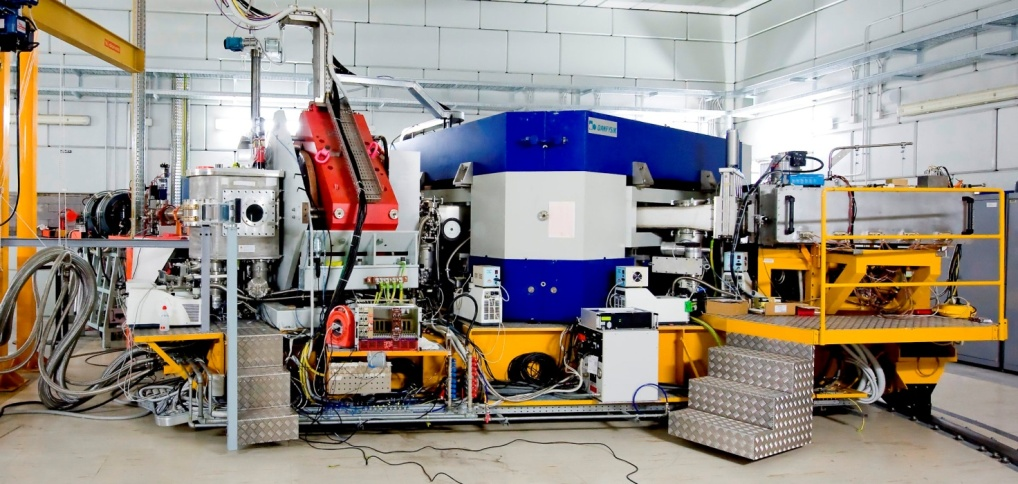
\includegraphics[width=\textwidth, keepaspectratio]{Grafici/magnex.jpg}
	\caption{Lo spettrometro magnetico MAGNEX.} \label{fig:magnex}
\end{figure}



%\clearpage 

\subsection{\iflanguage{italian}{Il rivelatore di piano focale}{The Focal Plane Detector}}

L'attuale FPD di MAGNEX, la cui rappresentazione schematica è riportata in Figura~\ref{fig:fpd}, è un sistema di rivelazione ibrido, costituito da un tracciatore a gas a bassa pressione e un muro di rivelatori a pad al silicio.
Esso è posizionato a 1.91~m dall'uscita del dipolo ed è inclinato di 59.2\textdegree{} rispetto ad un piano perpendicolare all'asse ottico, al fine di minimizzare gli effetti dovuti alle aberrazioni cromatiche\cite{cunsolo:nima01}.
Una finestra di mylar spessa 1.5~$\mu$m è utilizzata per contenere il gas, solitamente costituito da N35 isobutano.


\begin{figure} [!p]
	\centering
	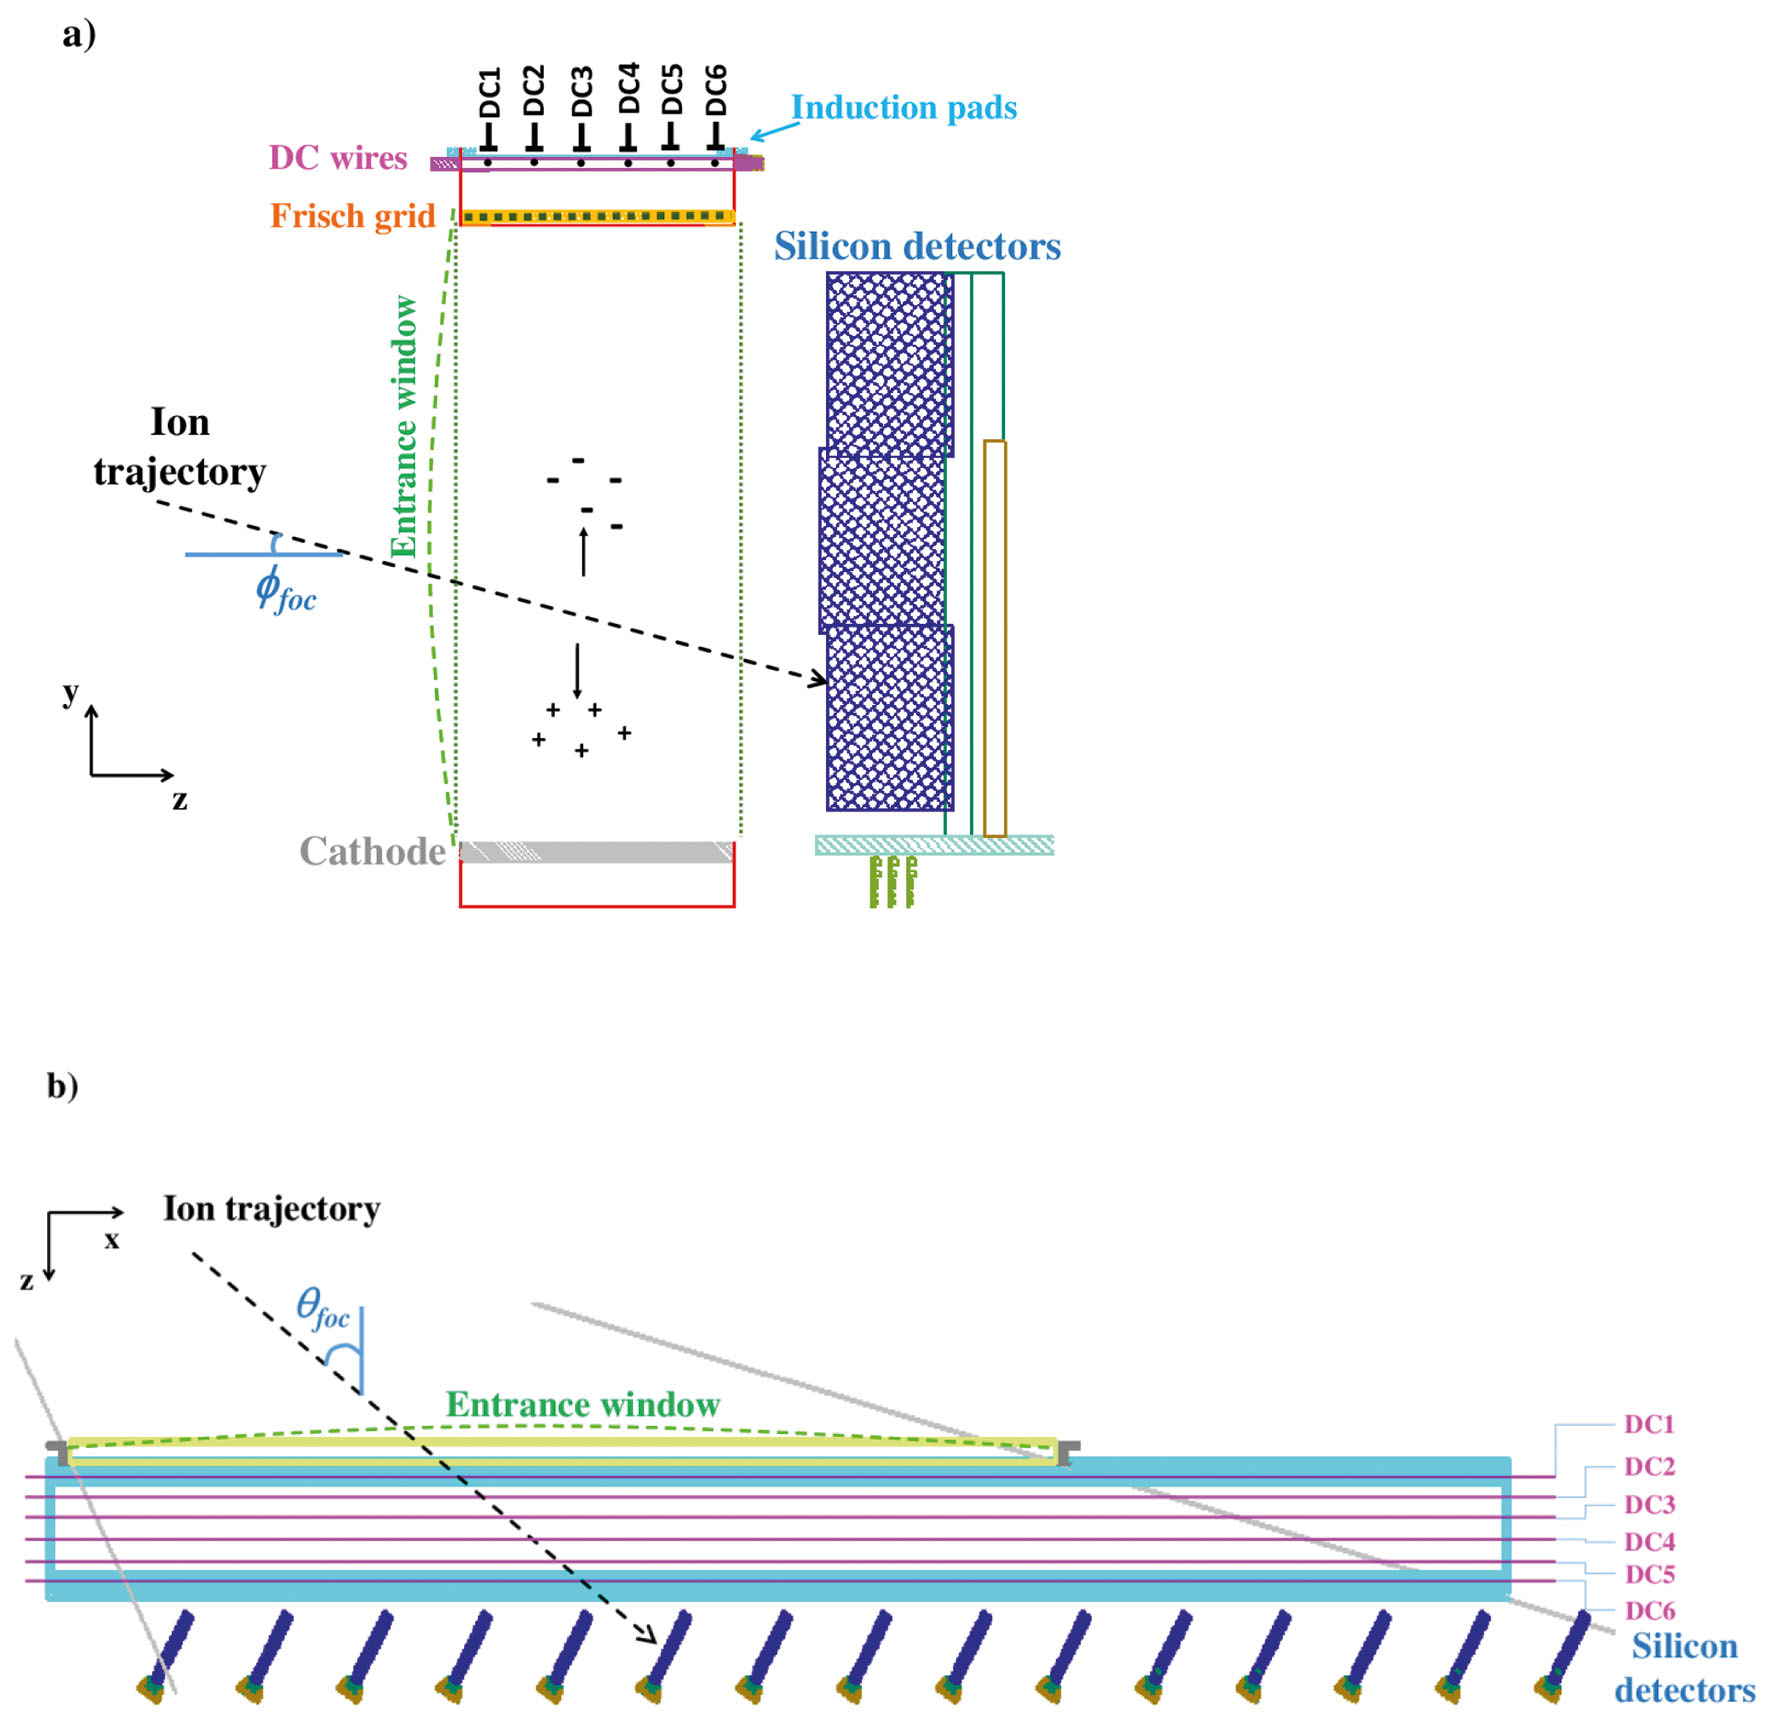
\includegraphics[width=\textwidth, keepaspectratio]{Grafici/fpd.png}
	\caption{Rappresentazione schematica del FPD: a) vista laterale; b) vista dall'alto. Figura tratta da~\cite{cappuzzello:epja18}.} \label{fig:fpd}
\end{figure}



%Il tracciatore a gas è formato da un sistema di sei fili al tungsteno placcati in oro, posti al di sotto di un anodo segmentato in pad. 
%Il tracciatore a gas lavora secondo il principio tipico delle camera a deriva.
%Il tracciatore a gas è essenzialmente una camera a deriva, in cui un sistema misto di fili e pad consente la misura dei quattro parametri necessari.
%Il tracciatore a gas, che consente la ricostruzione tridimensionale della traiettoria degli ioni, è formato da sei fili al tungsteno, indicati con DC\ped{\textit{i}}, e da un anodo segmentato in pad. 
%Al di sopra di ciascun filo si trova una fila di 224 pad
%Il tracciatore a gas è essenzialmente una camera a deriva, in cui un sistema costituito da sei fili (DC\ped{\textit{i}}) e da un anodo segmentato in pad consente la misura dei quattro parametri necessari per la ricostruzione tridimensionale della traccia.
%In particolare, al di sopra di ciascun filo è presente una fila di pad, le quali sono orientate parallelamente all'asse ottico.
Il tracciatore a gas, che consente la ricostruzione tridimensionale della traiettoria degli ioni, è formato da sei fili proporzionali (DC\ped{\textit{i}}) e da un anodo segmentato in sei file di pad, disposti in modo che sopra ogni filo ci sia una fila di pad.
I fili, sfruttando il principio di lavoro delle camere a deriva, danno una misura di sei posizioni verticali ($Y_i$), mentre le pad permettono di determinare sei posizioni orizzontali ($X_i$).
%Una griglia di Frisch è posta al di sotto dei fili, in quanto questi vengono anche utilizzati per misurare l'energia persa dagli ioni nel gas.
Dal che momento che i fili vengono anche utilizzati per misurare l'energia persa dagli ioni nel gas, una griglia di Frisch è posta al di sotto di essi.




Il muro di rivelatori al silicio è formato da 60 pad, disposte in 20 colonne contenenti 3 rivelatori ciascuna.
%Ogni pad ha un'area attiva di $70 \times 50$~mm\ap{2} ed è spessa 500~$\mu$m, sufficienti per fermare i prodotti di reazioni nel range energetico di interesse. 











